\documentclass[../report.tex]{subfiles}
\begin{document}
    
    \begin{frame}
        \frametitle{5: Tracking multiple targets}
        \begin{figure}[!htb]
            \centering
            \frame{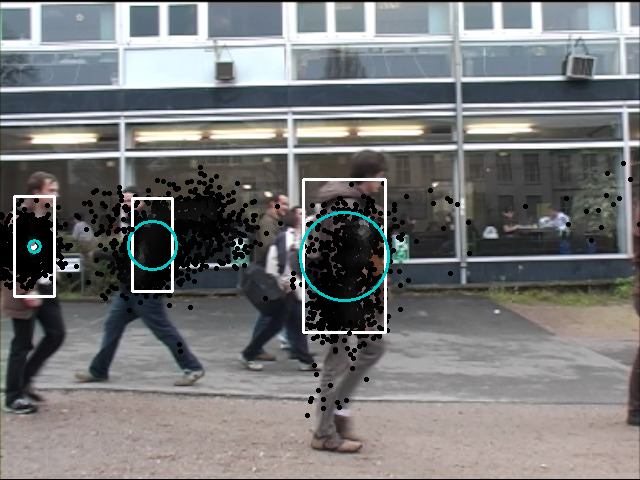
\includegraphics[keepaspectratio,height=0.65\textheight,width=0.45\textwidth]{ps5-5-a-1}}
            \caption{ps5-5-a-1}
        \end{figure}
    \end{frame}

    \begin{frame}
        \frametitle{5: Tracking multiple targets (cont.)}
        \begin{figure}[!htb]
            \centering
            \frame{
\includegraphics[keepaspectratio,height=0.65\textheight,width=0.45\textwidth]{ps5-5-a-2}}
            \caption{ps5-5-a-2}
        \end{figure}
    \end{frame}

    \begin{frame}
        \frametitle{5: Tracking multiple targets (cont.)}
        \begin{figure}[!htb]
            \centering
            \frame{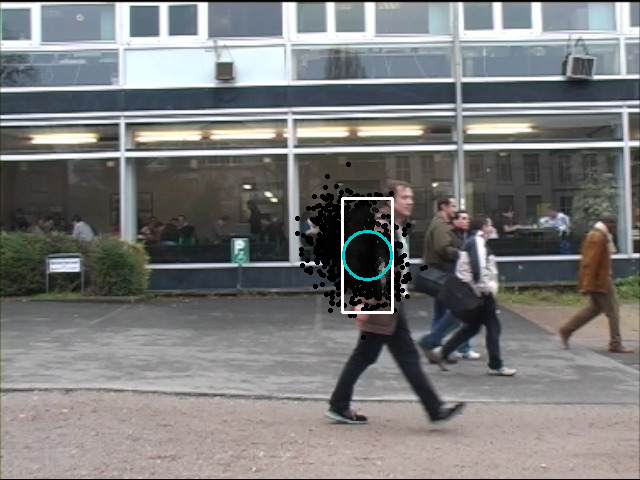
\includegraphics[keepaspectratio,height=0.65\textheight,width=0.45\textwidth]{ps5-5-a-3}}
            \caption{ps5-5-a-3}
        \end{figure}
    \end{frame}

    \begin{frame}[t]
        \frametitle{5: Text response}
        \begin{normalsize}
            \begin{itemize}
                \setlength\itemsep{1em}\fontsize{6pt}{6pt}

                \item[]{\textbf{\selectfont\textcolor{blue}{ Describe what you did. How different it was to use a KF vs PF? Which one worked best and why? Include details about any modifications you had to apply to handle multiple targets. }}}
                
                \item[]\textbf{\documentclass[../main.tex]{subfiles}
\begin{document}
    
    \begin{frame}
        \frametitle{5: AR in Video}
        \begin{figure}[!htb]
            \centering
            \subfloat[\small{ps3-5-a-1}]{\frame{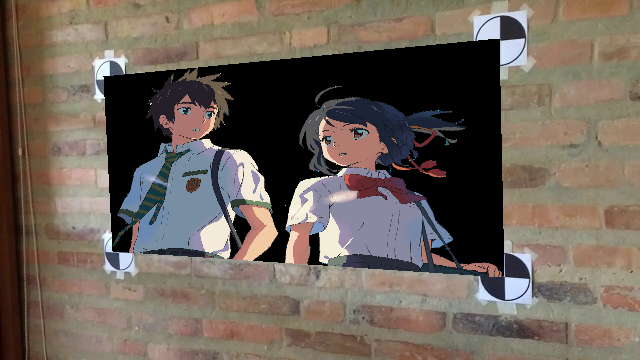
\includegraphics[keepaspectratio,height=0.65\textheight,width=0.45\textwidth]{ps3-5-a-1}}} \hspace{3em}
            \subfloat[\small{ps3-5-a-2}]{\frame{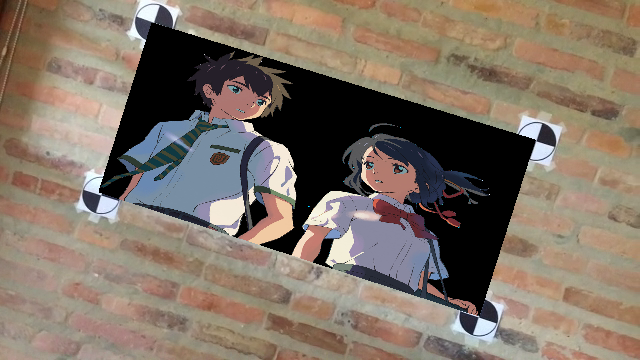
\includegraphics[keepaspectratio,height=0.65\textheight,width=0.45\textwidth]{ps3-5-a-2}}}
        \end{figure}
    \end{frame}

    \begin{frame}
        \frametitle{5: AR in Video (cont.)}
        \begin{table}[!htb]
        \centering
        \begin{tabular}{ c m{5cm} }
            \begin{minipage}{.45\textwidth}
                \frame{
\includegraphics[keepaspectratio,height=0.7\textheight,width=1\textwidth]{ps3-5-a-3}}\captionof{figure}{ps3-5-a-3}
            \end{minipage}
            &
            \begin{minipage}{.45\textwidth}
                \selectfont\textcolor{blue}{Youtube / Dropbox / etc. link:} \\
                % Please make sure that the link you submit is correct and can be viewed by a TA.
www.yourlink.com
            \end{minipage}
        \end{tabular}
        \end{table}
    \end{frame}

    \begin{frame}
        \frametitle{5: AR in Video (cont.)}
        \begin{figure}[!htb]
            \centering
            \subfloat[\small{ps3-5-a-4}]{\frame{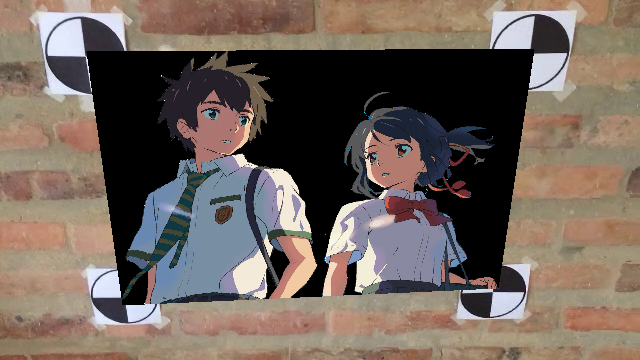
\includegraphics[keepaspectratio,height=0.65\textheight,width=0.45\textwidth]{ps3-5-a-4}}} \hspace{3em}
            \subfloat[\small{ps3-5-a-5}]{\frame{
\includegraphics[keepaspectratio,height=0.65\textheight,width=0.45\textwidth]{ps3-5-a-5}}}
        \end{figure}
    \end{frame}

    \begin{frame}
        \frametitle{5: AR in Video (cont.)}
        \begin{table}[!htb]
        \centering
        \begin{tabular}{ c m{5cm} }
            \begin{minipage}{.45\textwidth}
                \frame{
\includegraphics[keepaspectratio,height=0.7\textheight,width=1\textwidth]{ps3-5-a-6}}\captionof{figure}{ps3-5-a-6}
            \end{minipage}
            &
            \begin{minipage}{.45\textwidth}
                \selectfont\textcolor{blue}{Youtube / Dropbox / etc. link:} \\
                % Please make sure that the link you submit is correct and can be viewed by a TA.
www.yourlink.com
            \end{minipage}
        \end{tabular}
        \end{table}
    \end{frame}





    \begin{frame}
        \frametitle{5: Markers in Video}
        \begin{figure}[!htb]
            \centering
            \subfloat[\small{ps3-5-b-1}]{\frame{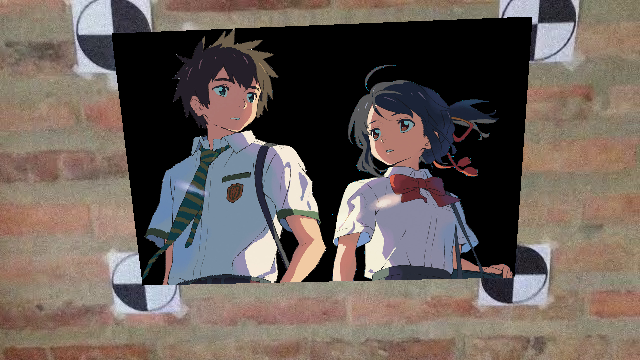
\includegraphics[keepaspectratio,height=0.65\textheight,width=0.45\textwidth]{ps3-5-b-1}}} \hspace{3em}
            \subfloat[\small{ps3-5-b-2}]{\frame{
\includegraphics[keepaspectratio,height=0.65\textheight,width=0.45\textwidth]{ps3-5-b-2}}}
        \end{figure}
    \end{frame}

    \begin{frame}
        \frametitle{5: Markers in Video (cont.)}
        \begin{table}[!htb]
        \centering
        \begin{tabular}{ c m{5cm} }
            \begin{minipage}{.45\textwidth}
                \frame{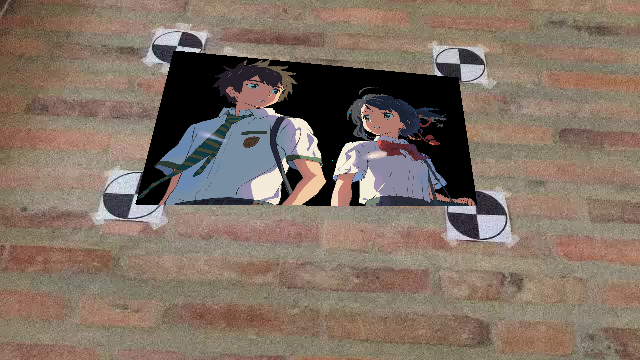
\includegraphics[keepaspectratio,height=0.7\textheight,width=1\textwidth]{ps3-5-b-3}}\captionof{figure}{ps3-5-b-3}
            \end{minipage}
            &
            \begin{minipage}{.45\textwidth}
                \selectfont\textcolor{blue}{Youtube / Dropbox / etc. link:} \\
                % Please make sure that the link you submit is correct and can be viewed by a TA.
www.yourlink.com
            \end{minipage}
        \end{tabular}
        \end{table}
    \end{frame}

    \begin{frame}
        \frametitle{5: Markers in Video (cont.)}
        \begin{figure}[!htb]
            \centering
            \subfloat[\small{ps3-5-b-4}]{\frame{
\includegraphics[keepaspectratio,height=0.65\textheight,width=0.45\textwidth]{ps3-5-b-4}}} \hspace{3em}
            \subfloat[\small{ps3-5-b-5}]{\frame{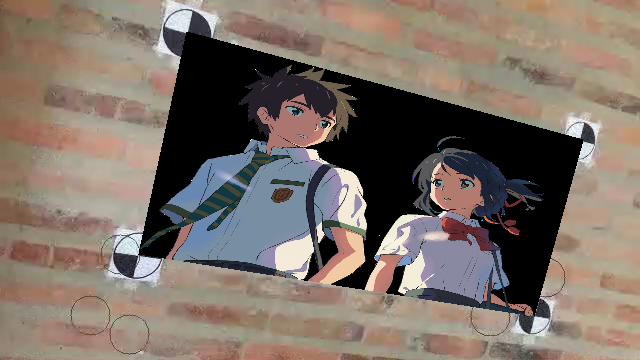
\includegraphics[keepaspectratio,height=0.65\textheight,width=0.45\textwidth]{ps3-5-b-5}}}
        \end{figure}
    \end{frame}

    \begin{frame}
        \frametitle{5: Markers in Video (cont.)}
        \begin{table}[!htb]
        \centering
        \begin{tabular}{ c m{5cm} }
            \begin{minipage}{.45\textwidth}
                \frame{
\includegraphics[keepaspectratio,height=0.7\textheight,width=1\textwidth]{ps3-5-b-6}}\captionof{figure}{ps3-5-b-6}
            \end{minipage}
            &
            \begin{minipage}{.45\textwidth}
                \selectfont\textcolor{blue}{Youtube / Dropbox / etc. link:} \\
                % Please make sure that the link you submit is correct and can be viewed by a TA.
www.yourlink.com
            \end{minipage}
        \end{tabular}
        \end{table}
    \end{frame}

\end{document}}
            \end{itemize}
        \end{normalsize}
    \end{frame}

\end{document}